\item At the moment \( t = 0 \) the force \( F = at \) is applied to a small body of mass \( m \) resting on a smooth horizontal plane (\( a \) is a constant).
    \begin{center}
        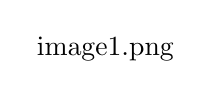
\begin{tikzpicture}
            \node at (0,0) {{image1.png}};
        \end{tikzpicture}
    \end{center}
    The permanent direction of this force forms an angle \( \alpha \) with the horizontal (Fig. 1.14). Find:
    \begin{enumerate}
        \item the velocity of the body at the moment of its breaking off the plane;
        \item the distance traversed by the body up to this moment.
    \end{enumerate}
\begin{solution}
    \begin{center}
        \begin{tikzpicture}
            \pic at (0, 0) {frame=3cm};
        \end{tikzpicture}
    \end{center}
    
    \begin{align*}
        \intertext{First of all let us draw the free body diagram for the small body of mass \(m\) and indicate \(x\)-axis along the horizontal plane and \(y\)-axis, perpendicular to it, as shown in the figure. Let the block break off the plane at \(t = t_0\), i.e., \(N = 0\).}
        N &= mg - at_0 \sin\alpha = 0\\
        t_0 &= \dfrac{mg}{a \sin\alpha}\\
        \intertext{From \(F_x = m a_x\) for the body under investigation}
        m \dfrac{dv_x}{dt} &= at \cos\alpha
        \intertext{Integrating within the limits for \(v(t)\)}
        \int_0^v m \, dv_x &= a \cos\alpha \int_0^t t \, dt \quad \text{(using Eq. 1)}
        \intertext{So,}
        v &= \dfrac{ds}{dt} = \dfrac{a \cos\alpha}{2m} t^2 \tag{2}
        \intertext{Integrating, Eq. (2) for \(s(t)\) we get}
        s &= \dfrac{a \cos\alpha}{2m} \dfrac{t^3}{3} \tag{3}
        \intertext{Using the value of \(t = t_0\) from Eq. (1), into Eqs. (2) and (3)}
        v &= \dfrac{mg^2 \cos\alpha}{2a \sin^2\alpha} \quad \text{and} \quad s = \dfrac{m^2g^3 \cos\alpha}{6 a^2 \sin^3\alpha}
    \end{align*}
\end{solution}
